\subsubsection{UC5 - Controllo delle unità}
\begin{figure}[h!]
    \centering
    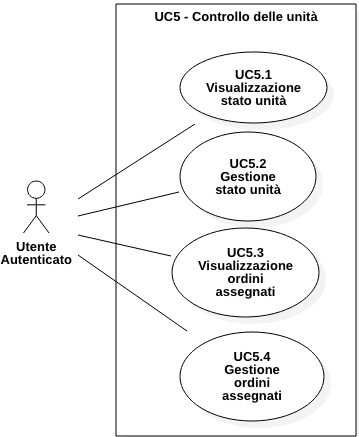
\includegraphics[width=10cm]{images/uc5.png}
    \caption{Diagramma UC5 - Controllo delle unità}
\end{figure}
\begin{itemize}
    \item \textbf{Attori primari:} utente autenticato;
    \item \textbf{Descrizione:} l'utente intende visualizzare e/o modificare le proprietà delle unità;
    \item \textbf{Scenario principale:} l'utente si trova in un area riservata nella quale viene presentata una lista delle unità collegate al sistema mediante il loro codice identificativo.\\
    Per una singola unità presente nella lista, l'utente in tempo reale può:
    \begin{itemize}
        \item visualizzare in dettaglio le proprietà dell'unità (UC5.1);
        \item gestire in dettaglio il comportamento dell'unità (UC5.2).
    \end{itemize}
    il tutto all'interno di un unico ambiente grafico dedicato.
    \item \textbf{Precondizione:} l'utente ha effettuato l'accesso al sistema;
    \item \textbf{Postcondizione:} l'utente visualizza le proprietà e modifica il comportamento di un'unità.
\end{itemize}
\newpage
    \subsubsection{UC5.1 - Visualizzazione unità}
    \begin{figure}[h!]
        \centering
        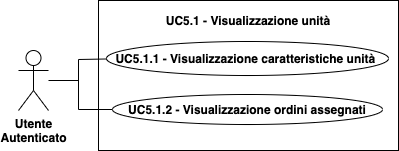
\includegraphics[width=10cm]{images/uc5.1.png}
        \caption{Diagramma UC5.1 - Visualizzazione unità}
    \end{figure}
    \begin{itemize}
        \item \textbf{Attori primari:} utente autenticato;
        \item \textbf{Descrizione:} l'utente intende visualizzare in dettaglio e in tempo reale le proprietà di un'unità;
        \item \textbf{Scenario principale:} l'utente visualizza:
        \begin{itemize}
            \item le caratteristiche dell'unità (UC5.1.1);
            \item la coda degli ordini assegnati all'unità (UC5.1.2).
        \end{itemize}
        \item \textbf{Precondizione:} l'utente accede all'ambiente grafico dedicato alle proprietà dell'unità;
        \item \textbf{Postcondizione:} l'utente visualizza in tempo reale le proprietà dell'unità.
    \end{itemize}

        \subsubsection{UC5.1.1 - Visualizzazione caratteristiche unità}
        \begin{itemize}
            \item \textbf{Attori primari:} utente autenticato;
            \item \textbf{Descrizione:} l'utente intende visualizzare le seguenti caratteristiche dell'unità:
            \begin{itemize}
                \item codice identificativo univoco;
                \item coordinate della posizione attuale all'interno della mappa;
                \item stato dell'unità che può essere:
                \begin{itemize}
                    \item \underline{Going to X}: dove X è il codice identificativo univoco del \glock{POI} (punto di consegna o base di ricarica) verso cui l'unità si sta dirigendo;
                    \item \underline{Stop}: l'unità, pur rimanendo accesa e connessa, rimane ferma nella sua posizione attuale;
                    \item \underline{Base}: come \underline{Stop} ma l'unità si trova nella base di ricarica pronta per ricevere nuovi ordini;
                    \item \underline{Error Y}: come \underline{Stop} ma l'unità si trova ferma a causa di un errore con codice identificativo univoco Y; alcuni errori potrebbero essere irreversibili e richiedere un intervento fisico sull'unità;
                    \item \underline{Disconnected}: il sistema non rileva l'unità che potrebbe essere spenta o disconnessa per motivazioni impreviste;
                \end{itemize}
                \item velocità attuale;
                \item direzione (suggerita dal sistema) del prossimo passo.
            \end{itemize}
            \item \textbf{Scenario principale:} l'utente prende visione dello stato dell'unità;
            \item \textbf{Precondizione:} l'utente naviga nell'ambiente grafico dedicato alle proprietà dell'unità;
            \item \textbf{Postcondizione:} l'utente visualizza in tempo reale le caratteristiche dell'unità.
        \end{itemize}

        \subsubsection{UC5.1.2 - Visualizzazione ordini assegnati}
        \begin{itemize}
            \item \textbf{Attori primari:} utente autenticato;
            \item \textbf{Descrizione:} l'utente intende visualizzare la coda degli ordini assegnati;
            \item \textbf{Scenario principale:} l'utente visualizza la coda degli ordini assegnati ovvero la lista dei \glock{POI} a cui effettuare la consegna prima di tornare alla base;
            \item \textbf{Precondizione:} l'utente naviga nell'ambiente grafico dedicato alle proprietà dell'unità;
            \item \textbf{Postcondizione:} l'utente visualizza in tempo reale la coda degli ordini assegnati all'unità.
        \end{itemize}


    \subsubsection{UC5.2 - Gestione unità}
    \begin{figure}[h!]
        \centering
        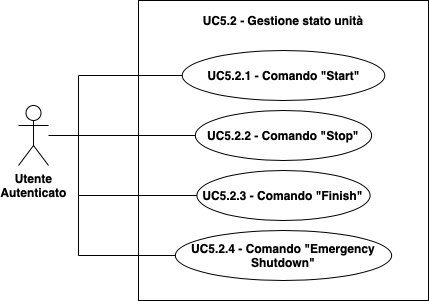
\includegraphics[width=10cm]{images/uc5.2.png}
        \caption{Diagramma UC5.2 - Gestione unità}
    \end{figure}
    \begin{itemize}
        \item \textbf{Attori primari:} utente autenticato;
        \item \textbf{Descrizione:} l'utente intende assegnare ordini all'unità o cambiarne lo stato;
        \item \textbf{Scenario principale:} l'utente impartisce determinati comandi per modificare lo stato dell'unità:
        \begin{itemize}
            \item Start (UC5.2.1);
            \item Stop (UC5.2.2);
            \item Go Back (UC5.2.3);
            \item Shutdown (UC5.2.4).
        \end{itemize}
        l'utente, inoltre, assegna (UC5.2.5) o elimina (UC5.2.6) ordini dalla coda degli ordini dell'unità;
        \item \textbf{Precondizione:} l'unità si trova in un determinato stato con una determinata coda degli ordini;
        \item \textbf{Postcondizione:} l'utente modifica in tempo reale lo stato dell'unità e la coda degli ordini.
    \end{itemize}

        \subsubsection{UC5.2.1 - Comando Start}
        \begin{itemize}
            \item \textbf{Attori primari:} utente autenticato;
            \item \textbf{Descrizione:} l'utente intende impostare lo stato dell'unità in modo che consegni tutti gli ordini assegnati per poi tornare alla base;
            \item \textbf{Scenario principale:} l'utente rende \underline{Going to X} il nuovo stato dell'unità;
            \item \textbf{Precondizione:} l'unità ha stato \underline{Base}, \underline{Stop} o un errore reversibile e la coda degli ordini contiene almeno un ordine;
            \item \textbf{Postcondizione:} l'unità ha stato \underline{Going to X}.
        \end{itemize}

        \subsubsection{UC5.2.2 - Comando Stop}
        \begin{itemize}
            \item \textbf{Attori primari:} utente autenticato;
            \item \textbf{Descrizione:} l'utente intende impostare lo stato dell'unità in modo che, pur rimanendo accesa e connessa, si fermi nella posizione attuale;
            \item \textbf{Scenario principale:} l'utente rende \underline{Stop} il nuovo stato dell'unità;
            \item \textbf{Precondizione:} l'unità ha stato \underline{Going to X};
            \item \textbf{Postcondizione:} l'unità ha stato \underline{Stop}.
        \end{itemize}

        \subsubsection{UC5.2.3 - Comando Go Back}
        \begin{itemize}
            \item \textbf{Attori primari:} utente autenticato;
            \item \textbf{Descrizione:} l'utente intende impostare lo stato dell'unità in modo che, indipendentemente dalla situazione attuale della coda degli ordini, ritorni alla base;
            \item \textbf{Scenario principale:} l'utente rende \underline{Going to B} il nuovo stato dell'unità, dove B è la base;
            \item \textbf{Precondizione:} l'unità ha stato \underline{Start}, \underline{Stop} o un errore reversibile;
            \item \textbf{Postcondizione:} l'unità ha stato \underline{Going to B} con B corrispondente alla base.
        \end{itemize}

        \subsubsection{UC5.2.4 - Comando Shutdown}
        \begin{itemize}
            \item \textbf{Attori primari:} utente autenticato;
            \item \textbf{Descrizione:} l'utente intende spegnere l'unità in modo immediato;
            \item \textbf{Scenario principale:} l'utente spegne l'unità in modo immediato ignorando stato attuale e qualsiasi ordine ancora assegnato;
            \item \textbf{Precondizione:} l'unità è accesa e connessa al sistema;
            \item \textbf{Postcondizione:} l'unità è spenta e per il sistema ha stato \underline{Disconnected}.
        \end{itemize}

        \subsubsection{UC5.4.5 - Assegnazione nuovo ordine}
        \begin{itemize}
            \item \textbf{Attori primari:} utente autenticato;
            \item \textbf{Descrizione:} l'utente intende accodare un nuovo ordine;
            \item \textbf{Scenario principale:} l'utente inserisce l'identificativo del \glock{POI} da visitare per effettuare la consegna;
            \item \textbf{Precondizione:} l'unità ha una coda degli ordini che non contiene l'ordine da inserire e si trova alla base;
            \item \textbf{Postcondizione:} l'unità ha la precedente coda degli ordini con accodato il nuovo ordine.
        \end{itemize}

        \subsubsection{UC5.4.6 - Eliminazione ordine assegnato}
        \begin{itemize}
            \item \textbf{Attori primari:} utente autenticato;
            \item \textbf{Descrizione:} l'utente intende eliminare un ordine in coda;
            \item \textbf{Scenario principale:} l'utente elimina l'ordine dalla coda indipendentemente dalla sua posizione all'interno di essa;
            \item \textbf{Precondizione:} l'unità ha una coda degli ordini con almeno un elemento e si trova alla base;
            \item \textbf{Postcondizione:} l'unità ha la precedente coda degli ordini ma senza l'ordine eliminato.
        \end{itemize}
